\documentclass[UTF8,a4paper,12pt,fontset=none]{ctexart}
\usepackage[margin=2.5cm]{geometry}
\usepackage{amsmath,amssymb}
\usepackage{graphicx}
\usepackage{booktabs}
\usepackage{longtable}
\usepackage{array}
\usepackage{float}
\usepackage{caption}
\usepackage{xcolor}
\usepackage{hyperref}
\usepackage{setspace}
\usepackage{listings}
\usepackage{enumitem}
\setCJKmainfont{Noto Serif CJK SC}
\setCJKsansfont{Noto Sans CJK SC}
\setCJKmonofont{Noto Sans Mono CJK SC}
\setstretch{1.32}
\setlength{\parskip}{0.35em}
\setlist{itemsep=0.15em, topsep=0.25em}
\emergencystretch=2em
\ctexset{
    section = {name = {}, number = \arabic{section}, aftername = \quad},
    subsection = {name = {}, number = \arabic{section}.\arabic{subsection}, aftername = \quad}
}
\hypersetup{
    colorlinks=true,
    linkcolor=blue,
    citecolor=blue,
    urlcolor=blue
}
\lstset{
    basicstyle=\ttfamily\footnotesize,
    breaklines=true,
    frame=single,
    columns=fullflexible,
    keepspaces=true
}
\graphicspath{{../../}{../../report_assets/Experiment2_ADMM_ASGO/}}

\title{结合 ADMM 与 ASGO 的稀疏 PINN 优化实验}
\author{}
\date{}

\begin{document}
\maketitle
\tableofcontents
\newpage


\section{摘要}

本实验围绕课程中“目标函数 + 非光滑正则项”的优化建模要求，设计并实现了一个 ADMM-ASGO 稀疏 PINN 训练实验。实验对象沿用当前项目已有的 Burgers 方程物理信息神经网络（PINN）管线，核心问题是：能否把神经网络训练中的光滑 PINN 损失与非光滑 L1 稀疏正则项分开处理，使模型最终得到严格为零的权重，同时保持物理解拟合误差处在可接受范围内？

本文将矩阵权重训练写成变量分裂形式：

\[
\min_{\theta,z}\mathcal L_{\mathrm{PINN}}(\theta)+\lambda\|z\|_1,\quad \mathrm{s.t.}\ \theta=z.
\]

其中 $\mathcal L_{\mathrm{PINN}}$ 是 Burgers 方程 PDE 残差、初值条件和边界条件组成的光滑非凸损失；$\|z\|_1$ 是非光滑稀疏正则项。实验采用 ASGO 作为 ADMM 中 $\theta$ 子问题的结构化梯度优化器，用软阈值算子求解 $z$ 子问题，并通过对偶变量更新维持 $\theta$ 与 $z$ 的一致性。

正式实验运行 30000 epoch、3 个随机种子，对比 Standard Adam、ConFIG、M-ConFIG、ASGO、Adam + L1、ASGO + L1 和 ADMM-ASGO。结果显示，普通 L1 惩罚和 ASGO + L1 在有限步梯度训练后均没有产生严格零权重；ADMM-ASGO 则得到 26.58\% 的矩阵权重稀疏率，非零矩阵权重从 10150 个减少到约 7452 个，同时 run-test MSE 为 $2.3000\times 10^{-4}$。这说明 ADMM 的近端分裂确实能产生普通 L1 梯度惩罚难以得到的严格稀疏性，但稀疏化会带来一定精度损失，体现了 PINN 物理残差拟合与模型压缩之间的折中。

本实验不声称超过 ASGO、ConFIG 或 PINN 原方法，而是验证一个明确的优化思想：将 ASGO 的结构化梯度优化能力嵌入 ADMM 的光滑子问题，并用软阈值步骤显式产生稀疏神经网络权重。

\section{研究背景与问题动机}

\subsection{为什么关心稀疏化和优化方法}

Villalobos 等人在 *Will we run out of data?* 中讨论了机器学习数据规模扩张的边界，并指出如果当前趋势持续，大模型训练可能在未来几年接近公开高质量人类文本数据的存量上限。这个背景说明，模型能力的提升不能只依赖“更多数据、更大模型”的单一路径，还需要依靠更高效的优化、更好的结构化更新、更强的正则化和更可控的约束建模。

类似问题也出现在科学机器学习中。以 PINN 为例，训练目标不仅要拟合数据，还要满足微分方程、初值条件和边界条件。它通常具有以下困难：

\begin{enumerate}
\item PDE 残差和边界/初值误差可能存在梯度冲突；
\item 训练目标是高非凸的，损失曲面复杂；
\item 参数量虽然小于大语言模型，但对科学计算任务而言仍有压缩和解释需求；
\item 如果直接加入 L1 正则，梯度下降往往只能让参数变小，不一定产生严格零值。
\end{enumerate}

因此，本实验选择“ADMM + ASGO + PINN 稀疏化”作为研究对象。ADMM 擅长把非光滑项与光滑项分裂，ASGO 擅长利用矩阵权重的结构化梯度信息，PINN 则提供一个有物理意义、可验证的非凸神经网络训练场景。

\subsection{相关文献}

ASGO（Adaptive Structured Gradient Optimization）由 An 等人在 NeurIPS 2025 提出。该方法关注二维矩阵权重的结构化梯度更新，相比 Adam 的逐元素自适应缩放，ASGO 使用矩阵层面的预条件信息来调整更新方向。本实验在代码复现中引入 ASGO 的公开实现作为结构化优化器参考，并固定外部依赖版本，以保证训练结果和分析结果可以被稳定复现。具体代码版本记录在实验脚本和 \texttt{external/ASGO} 目录中。

Zhou 等人在 2026 年 Nature Machine Intelligence 发表 *Preconditioned inexact stochastic ADMM for deep models*，说明 ADMM 仍然是深度模型优化中的活跃方向，尤其适合变量分裂、一致性约束、预条件更新和大规模随机优化。本文不复现该论文的大规模深度模型实验，而是在 Burgers PINN 上实现一个小规模但完整可复现的 ADMM 稀疏训练流程。

ConFIG 和 M-ConFIG 是当前仓库已有的 PINN 多目标梯度优化基线。它们主要处理 PINN 中不同损失分量之间的梯度冲突。本实验把它们作为精度基线，帮助判断 ADMM-ASGO 的误差水平。

\section{ADMM 理论推导}

\subsection{ADMM 的基本思想：为什么要把问题拆开}

ADMM 是 Alternating Direction Method of Multipliers，即交替方向乘子法。它的出发点不是把简单问题故意写复杂，而是处理一类普通梯度下降很难直接处理的问题：目标函数里同时出现了适合求梯度的光滑项、不能在所有点求导的非光滑项，或者还带有必须严格满足的约束。

以本实验关心的稀疏训练为例，神经网络的 PINN 损失可以通过反向传播求梯度，因此适合交给 Adam、ASGO 等梯度型优化器；但 L1 正则项含有绝对值，单变量函数 $|x|$ 在 $x=0$ 处有尖角，没有唯一导数。如果把二者硬塞进同一个普通梯度下降过程，优化器通常只能把权重推得很小，却不容易让权重精确等于 0。对模型压缩而言，$10^{-5}$ 这样的小权重仍然需要存储和计算，而严格的 0 才能对应真正的稀疏结构。

这就是 ADMM 的算子分裂思想：把一个变量复制成两个变量，让其中一个变量负责光滑损失，另一个变量负责非光滑正则项，再用等式约束要求二者最终一致。这个辅助变量不是新的物理参数，而是原变量的一份优化副本。例如在稀疏神经网络中，可以把 $z$ 理解为权重 $\theta$ 的稀疏副本：$\theta$ 负责拟合 PDE，$z$ 负责被 L1 正则截断成稀疏形式，约束 $\theta=z$ 则保证二者最后描述的是同一个模型。

为了处理约束，ADMM 从增广拉格朗日方法出发。对约束 $Ax+Bz=c$，普通拉格朗日函数会引入乘子 $y$；增广拉格朗日函数进一步加入二次惩罚项：

\[
L_\rho(x,z,y)=f(x)+g(z)+y^T(Ax+Bz-c)+\frac{\rho}{2}\|Ax+Bz-c\|_2^2.
\]

这里 $y$ 是拉格朗日乘子，$\rho>0$ 是惩罚参数。为了让公式更简洁，常定义缩放对偶变量 $u=y/\rho$。利用配方法，含有 $y$ 的两项可写成：

\[
y^Tr+\frac{\rho}{2}\|r\|_2^2=\frac{\rho}{2}\left\|r+\frac{y}{\rho}\right\|_2^2-\frac{1}{2\rho}\|y\|_2^2,
\]

其中 $r=Ax+Bz-c$。最后一项与 $x,z$ 无关，在交替最小化时可视为常数，于是公式中自然出现了 $u$。因此，$u$ 并不是凭空出现的量，而是缩放后的拉格朗日乘子，用来记录和累积当前两个变量违反约束的程度。

ADMM 的通用套路可以概括为三步：先固定 $z,u$ 更新 $x$，再固定 $x,u$ 更新 $z$，最后根据约束残差更新 $u$。它的价值在于：$x$ 子问题可以交给适合光滑项的优化方法，$z$ 子问题可以交给非光滑项的近端算子，约束一致性则由对偶变量持续调节。

\subsection{问题一：$\min f(x)+\gamma\|x\|_1,\ x\in X$}

这个问题是本实验 ADMM-ASGO 的理论原型。$f(x)$ 表示主要训练损失，例如神经网络中的 MSE、PINN 残差损失或交叉熵等。我们称它为光滑项，是因为它在优化过程中通常可由自动微分计算梯度，并可用 Adam、SGD、ASGO 等方法更新。$\gamma\|x\|_1$ 是 L1 正则项，其中 $\|x\|_1=\sum_i |x_i|$。绝对值函数在 0 点不可导，因此这一项是非光滑项。

一个自然问题是：为什么不用光滑的 L2 正则？原因是 L2 正则主要产生权重衰减，它倾向于把参数连续地缩小，但通常不会把参数直接变成严格的 0。L1 正则虽然带来非光滑困难，却具有诱导稀疏性的能力。更准确地说，在 ADMM 或近端梯度这类方法中，L1 的稀疏性不是靠普通梯度下降慢慢“降到 0”，而是由软阈值近端算子直接截断得到。

为了把光滑损失和非光滑正则分开，引入辅助变量 $z$，令它承担 L1 正则：

\[
\min_{x,z} f(x)+\gamma\|z\|_1,\quad \mathrm{s.t.}\ x-z=0,\ x\in X.
\]

这个问题与原问题等价，因为约束 $x=z$ 成立时，$\|z\|_1$ 就等于 $\|x\|_1$。但改写后两个任务被拆开了：$x$ 负责优化 $f$，$z$ 负责处理 L1。

对约束 $x-z=0$ 写增广拉格朗日函数，并使用缩放对偶变量 $u$，得到：

\[
\mathcal L_\rho(x,z,u)=f(x)+\gamma\|z\|_1+\frac{\rho}{2}\|x-z+u\|_2^2.
\]

第一步，固定 $z^k,u^k$ 更新 $x$：

\[
x^{k+1}=\arg\min_{x\in X}\left(f(x)+\frac{\rho}{2}\|x-z^k+u^k\|_2^2\right).
\]

此时目标函数里已经没有 L1 尖角，只剩下原始光滑损失和一个光滑二次惩罚项。对神经网络而言，这一步可以用反向传播和 ASGO/Adam 近似求解。二次项的作用是提醒 $x$ 不要离上一轮稀疏副本 $z^k$ 太远。

第二步，固定 $x^{k+1},u^k$ 更新 $z$：

\[
z^{k+1}=\arg\min_z\left(\gamma\|z\|_1+\frac{\rho}{2}\|x^{k+1}-z+u^k\|_2^2\right).
\]

令 $c=x^{k+1}+u^k$，上式等价于：

\[
z^{k+1}=\arg\min_z\left(\gamma\|z\|_1+\frac{\rho}{2}\|z-c\|_2^2\right).
\]

这个问题按坐标可分。对单个坐标 $z_i$，需要最小化：

\[
\gamma |z_i|+\frac{\rho}{2}(z_i-c_i)^2.
\]

当 $z_i>0$ 时，一阶条件为 $\gamma+\rho(z_i-c_i)=0$，得到 $z_i=c_i-\gamma/\rho$，并要求 $c_i>\gamma/\rho$；当 $z_i<0$ 时，一阶条件为 $-\gamma+\rho(z_i-c_i)=0$，得到 $z_i=c_i+\gamma/\rho$，并要求 $c_i<-\gamma/\rho$；当 $|c_i|\le \gamma/\rho$ 时，最优解落在尖点 $z_i=0$。因此闭式解为软阈值算子：

\[
z^{k+1}=S_{\gamma/\rho}(x^{k+1}+u^k),
\]

\[
S_\kappa(a)=\mathrm{sign}(a)\max(|a|-\kappa,0).
\]

这一步解释了 L1 稀疏性的来源：只要 $|a|\le \kappa$，对应坐标就被精确置为 0。严格零值不是普通梯度下降碰巧得到的，而是软阈值公式中的 $\max(\cdot,0)$ 明确产生的。

第三步，更新缩放对偶变量：

\[
u^{k+1}=u^k+x^{k+1}-z^{k+1}.
\]

其中 $x^{k+1}-z^{k+1}$ 是当前约束残差。如果 $x$ 和 $z$ 差得较多，$u$ 会把这种分歧累积下来，在下一轮更新中改变二次惩罚中心，推动二者逐渐一致。

\subsection{问题二：$\min\|Cx-b\|_1,\ x\in\mathbb R^n$}

第二个问题可以理解为鲁棒线性拟合。普通最小二乘最小化 $\|Cx-b\|_2^2$，对离群点很敏感；L1 残差 $\|Cx-b\|_1$ 对异常值更稳健，但问题在于绝对值外面套着线性变换 $Cx-b$，直接处理并不方便。

令残差副本：

\[
z=Cx-b.
\]

原问题等价改写为：

\[
\min_{x,z}\|z\|_1,\quad \mathrm{s.t.}\ Cx-b-z=0.
\]

这里 $x$ 负责满足线性模型，$z$ 负责表示残差并接受 L1 处理。缩放形式的增广拉格朗日函数为：

\[
\mathcal L_\rho(x,z,u)=\|z\|_1+\frac{\rho}{2}\|Cx-b-z+u\|_2^2.
\]

第一步，固定 $z^k,u^k$ 更新 $x$：

\[
x^{k+1}=\arg\min_x\frac{\rho}{2}\|Cx-b-z^k+u^k\|_2^2.
\]

去掉正系数 $\rho/2$ 不影响最优解，该问题就是一个最小二乘问题：

\[
\min_x\|Cx-(b+z^k-u^k)\|_2^2.
\]

对 $x$ 求导并令其为 0：

\[
2C^T(Cx-(b+z^k-u^k))=0.
\]

于是得到正规方程：

\[
C^TCx=C^T(b+z^k-u^k).
\]

若 $C^TC$ 可逆，则闭式解为：

\[
x^{k+1}=(C^TC)^{-1}C^T(b+z^k-u^k).
\]

若不可逆，可以使用伪逆或阻尼最小二乘。这里的重点是，变量分裂后，原本含 L1 的问题被拆成了一个标准二次最小二乘子问题。

第二步，固定 $x^{k+1},u^k$ 更新 $z$：

\[
z^{k+1}=\arg\min_z\left(\|z\|_1+\frac{\rho}{2}\|Cx^{k+1}-b-z+u^k\|_2^2\right).
\]

令 $c=Cx^{k+1}-b+u^k$，得到：

\[
z^{k+1}=\arg\min_z\left(\|z\|_1+\frac{\rho}{2}\|z-c\|_2^2\right).
\]

与问题一相同，它的解是软阈值：

\[
z^{k+1}=S_{1/\rho}(Cx^{k+1}-b+u^k).
\]

第三步，更新对偶变量：

\[
u^{k+1}=u^k+Cx^{k+1}-b-z^{k+1}.
\]

这一项累积的是约束 $Cx-b-z=0$ 的违反程度。通过不断更新 $u$，ADMM 让 $z$ 既能保持 L1 鲁棒处理，又逐渐与真实残差 $Cx-b$ 保持一致。

\subsection{问题三：$\min\|x\|_1,\ \mathrm{s.t.}\ Cx=b$}

第三个问题是带硬约束的稀疏优化。它常见于压缩感知：当线性方程 $Cx=b$ 有很多解时，希望从中选出非零元素尽可能少的一个。这个问题比问题一多了硬约束 $Cx=b$，要求最终解必须严格满足线性方程。

引入辅助变量 $z=x$，让 $z$ 负责 L1 稀疏项，让 $x$ 负责满足线性约束：

\[
\min_{x,z}\|z\|_1,\quad \mathrm{s.t.}\ x-z=0,\ Cx=b.
\]

这里我们把 $x=z$ 放进 ADMM 的增广拉格朗日项，把 $Cx=b$ 保留为 $x$ 子问题中的硬约束。缩放形式为：

\[
\mathcal L_\rho(x,z,u)=\|z\|_1+\frac{\rho}{2}\|x-z+u\|_2^2,\quad \mathrm{s.t.}\ Cx=b.
\]

第一步，固定 $z^k,u^k$ 更新 $x$：

\[
x^{k+1}=\arg\min_{Cx=b}\frac{\rho}{2}\|x-z^k+u^k\|_2^2.
\]

令 $v=z^k-u^k$，则问题变为：

\[
x^{k+1}=\arg\min_{Cx=b}\frac{\rho}{2}\|x-v\|_2^2.
\]

它的几何意义是：在满足 $Cx=b$ 的仿射空间中，寻找离点 $v$ 最近的点，也就是把 $v$ 投影到约束集合上。为了推导闭式解，引入内层拉格朗日乘子 $\alpha$：

\[
\mathcal J(x,\alpha)=\frac{\rho}{2}\|x-v\|_2^2+\alpha^T(Cx-b).
\]

对 $x$ 求导并令其为 0：

\[
\rho(x-v)+C^T\alpha=0.
\]

因此：

\[
x=v-\frac{1}{\rho}C^T\alpha.
\]

将它代回硬约束 $Cx=b$：

\[
C\left(v-\frac{1}{\rho}C^T\alpha\right)=b.
\]

整理得到：

\[
Cv-\frac{1}{\rho}CC^T\alpha=b,
\]

\[
\frac{1}{\rho}\alpha=(CC^T)^{-1}(Cv-b),
\]

其中假设 $CC^T$ 可逆。代回 $x$ 的表达式：

\[
x=v-C^T(CC^T)^{-1}(Cv-b).
\]

展开后得到：

\[
x^{k+1}=\left(I-C^T(CC^T)^{-1}C\right)(z^k-u^k)+C^T(CC^T)^{-1}b.
\]

这个公式中出现 $b$ 并不突兀，因为 $b$ 正是硬约束 $Cx=b$ 的右端项，投影点必须由它决定。

第二步，固定 $x^{k+1},u^k$ 更新 $z$：

\[
z^{k+1}=\arg\min_z\left(\|z\|_1+\frac{\rho}{2}\|x^{k+1}-z+u^k\|_2^2\right).
\]

这仍然是 L1 近端问题，因此：

\[
z^{k+1}=S_{1/\rho}(x^{k+1}+u^k).
\]

第三步，更新对偶变量：

\[
u^{k+1}=u^k+x^{k+1}-z^{k+1}.
\]

这个问题展示了 ADMM 的另一种价值：硬约束由投影步骤精确处理，稀疏性由软阈值步骤处理，二者不需要混在同一个难解目标里。

\subsection{与本实验的对应关系}

本实验使用的是问题一的思想。神经网络权重 $\theta$ 对应上面的 $x$，稀疏副本 $z$ 对应被 L1 正则处理的变量，PINN 损失 $\mathcal L_{\mathrm{PINN}}(\theta)$ 对应光滑项 $f(x)$。ADMM-ASGO 的 $\theta$ 子问题用 ASGO 近似求解，$z$ 子问题用软阈值精确求解，$u$ 则记录 $\theta$ 与 $z$ 的一致性残差。

因此，本文的方法不是简单地“给 PINN 损失加一个 L1 项”，而是把 L1 项从普通梯度下降中分离出来，交给它真正适合的近端算子处理。这也是 ADMM-ASGO 能产生严格零权重，而 Adam + L1 和 ASGO + L1 在本实验中没有产生严格零权重的根本原因。

\section{方法：ADMM-ASGO 稀疏 PINN}

\subsection{Burgers PINN 训练目标}

Burgers 方程 PINN 使用神经网络 $u_\theta(x,t)$ 近似 PDE 解。训练损失由内部物理残差、初值条件和边界条件组成：

\[
\mathcal L_{\mathrm{PINN}}(\theta)=\mathcal L_{\mathrm{PDE}}(\theta)+\mathcal L_{\mathrm{BI}}(\theta).
\]

为了引入稀疏性，本文只对 \texttt{nn.Linear.weight} 这类二维矩阵权重做 L1 稀疏化，不对 bias 做稀疏化。原因有两点：第一，ASGO 本身主要适配二维矩阵权重；第二，bias 参数数量很少，强行稀疏化对压缩收益有限，却可能影响 PINN 的表达稳定性。

最终优化模型为：

\[
\min_{\theta,z}\mathcal L_{\mathrm{PINN}}(\theta)+\lambda\|z\|_1,\quad \mathrm{s.t.}\ \theta=z.
\]

\subsection{ADMM-ASGO 迭代}

在每个训练 epoch 中，ADMM-ASGO 执行如下步骤。

第一步，$\theta$ 子问题：

\[
\theta^{k+1}\approx \arg\min_\theta \mathcal L_{\mathrm{PINN}}(\theta)+\frac{\rho}{2}\|\theta-z^k+u^k\|_2^2.
\]

该子问题是光滑非凸问题。本文不精确求解它，而是用 ASGO 做一次结构化梯度更新。具体实现中，矩阵权重走 ASGO，bias 和一维参数走 Adam。

第二步，$z$ 子问题：

\[
z^{k+1}=S_{\lambda/\rho}(\theta^{k+1}+u^k).
\]

软阈值是产生严格零权重的关键。如果某个权重的绝对值小于阈值 $\lambda/\rho$，它会被直接置为 0。

第三步，对偶变量更新：

\[
u^{k+1}=u^k+\theta^{k+1}-z^{k+1}.
\]

训练结束时，把 $z$ 写回网络权重后保存，因此最终的 \texttt{trained\_network\_weights.pt} 是稀疏模型，而不是仅在训练日志中记录的临时稀疏变量。

\subsection{代码实现}

本实验新增 \texttt{experiments/PINN/lib\_pinns/sparse\_trainers.py}，主要包含：

\begingroup
\small
\begin{longtable}{p{0.25\textwidth}p{0.65\textwidth}}
\toprule
组件 & 作用 \\
\midrule
\texttt{soft\_threshold} & L1 近端软阈值算子 \\
\texttt{sparse\_named\_parameters} & 筛选需要稀疏化的二维矩阵权重 \\
\texttt{LocalASGO} & 从 ASGO 官方实现适配的本地矩阵优化器 \\
\texttt{HybridOptimizer} & 矩阵权重使用 ASGO，一维参数使用 Adam \\
\texttt{L1PenaltyTrainerBasis} & Adam + L1 基线 \\
\texttt{ASGOTrainerBasis} & ASGO 基线 \\
\texttt{ASGOL1TrainerBasis} & ASGO + L1 基线 \\
\texttt{ADMMASGOTrainerBasis} & ADMM-ASGO 主方法 \\
\bottomrule
\end{longtable}
\endgroup


\texttt{tools/Experiment2\_ADMM\_ASGO/run\_burgers\_experiments.py} 新增方法：

\begin{lstlisting}
standard config mconfig asgo adam_l1 asgo_l1 admm_asgo
\end{lstlisting}

\texttt{tools/Experiment2\_ADMM\_ASGO/analyze\_burgers\_results.py} 新增以下分析能力：

\begin{enumerate}
\item 读取新增方法目录；
\item 统计全局矩阵权重稀疏率；
\item 统计逐层稀疏率；
\item 统计非零矩阵权重数量；
\item 读取 ADMM primal residual 和 dual residual；
\item 输出收敛曲线、精度-稀疏度图、全局稀疏率图、逐层稀疏率图、Burgers 预测与误差热力图。
\end{enumerate}

\section{实验设置}

\subsection{数据、网络与训练配置}

实验沿用当前仓库已有的 Burgers 1D PINN 管线：

\begingroup
\small
\begin{longtable}{p{0.25\textwidth}p{0.65\textwidth}}
\toprule
项目 & 设置 \\
\midrule
方程 & 一维 Burgers 方程 \\
网络 & \texttt{BurgersNet} \\
输入 & $(x,t)$ \\
输出 & $u(x,t)$ \\
内部采样点 & 10000 \\
初值点 & 250 \\
边界点 & 250 \\
训练采样 & Latin hypercube \\
验证/测试数据 & \texttt{experiments/PINN/data/burgers/simulation\_data.npy} \\
正式训练 epoch & 30000 \\
随机种子数量 & 3 \\
ADMM 参数 & $\lambda=10^{-5},\ \rho=10^{-2}$ \\
ASGO 矩阵逆根迭代步 & 5 \\
\bottomrule
\end{longtable}
\endgroup


\subsection{对比方法}

\begingroup
\small
\begin{longtable}{p{0.25\textwidth}p{0.65\textwidth}}
\toprule
方法 & 说明 \\
\midrule
Standard Adam & 当前 PINN 标准 Adam 训练 \\
ConFIG & 当前仓库已有的无冲突梯度基线 \\
M-ConFIG & 当前仓库已有的改进 ConFIG 基线 \\
ASGO & 矩阵权重使用 ASGO，bias 使用 Adam \\
Adam + L1 & 在 Adam PINN 损失上直接加 L1 惩罚 \\
ASGO + L1 & 在 ASGO PINN 损失上直接加 L1 惩罚 \\
ADMM-ASGO & ASGO 解光滑子问题，软阈值解 L1 子问题 \\
\bottomrule
\end{longtable}
\endgroup


\subsection{运行命令}

正式全量实验命令为：

\begin{lstlisting}
python3 tools/Experiment2_ADMM_ASGO/run_burgers_experiments.py \
  --epochs 30000 \
  --num-run 3 \
  --methods standard config mconfig asgo adam_l1 asgo_l1 admm_asgo \
  --device cuda:0 \
  --save-path ./PINN_trained/Burgers/Experiment2_ADMM_ASGO/ \
  --name-suffix _exp2_full \
  --save-epoch 30000 \
  --final-record-epoch 500 \
  --asgo-matalg-steps 5 \
  --admm-lambda 1e-5 \
  --admm-rho 1e-2 \
  --parallel-methods 4
\end{lstlisting}

分析命令为：

\begin{lstlisting}
python3 tools/Experiment2_ADMM_ASGO/analyze_burgers_results.py \
  --run-root PINN_trained/Burgers/Experiment2_ADMM_ASGO \
  --methods standard_30000_exp2_full config_30000_exp2_full mconfig_30000_exp2_full asgo_30000_exp2_full adam_l1_30000_exp2_full asgo_l1_30000_exp2_full admm_asgo_30000_exp2_full \
  --out-dir report_assets/Experiment2_ADMM_ASGO \
  --device cuda:0
\end{lstlisting}

\subsection{检查项}

正式实验前后完成了以下检查：

\begin{enumerate}
\item \texttt{soft\_threshold} 对正数、负数、零和小于阈值的数值输出正确；
\item ADMM 状态变量 \texttt{z/u} 与目标权重的 shape、device、dtype 保持一致；
\item 稀疏率统计只统计被 ADMM 管理的矩阵权重，不统计 bias；
\item 训练目录中生成 \texttt{training\_event.log}、\texttt{trained\_network\_weights.pt}、\texttt{configs.yaml}；
\item 分析脚本能读取新增方法目录并生成 JSON 汇总和报告图表；
\item ADMM-ASGO 最终保存权重中确实存在严格零值。
\end{enumerate}

\section{实验结果}

\subsection{总体数值结果}

下表为 30000 epoch、3 个随机种子的均值和标准差。稀疏率只统计二维矩阵权重，因此所有方法的矩阵权重总数均为 10150。

\begingroup
\scriptsize
\begin{longtable}{p{0.15\textwidth}p{0.13\textwidth}p{0.13\textwidth}p{0.13\textwidth}p{0.13\textwidth}p{0.13\textwidth}p{0.13\textwidth}}
\toprule
方法 & Final validation MSE & Best validation MSE & Run-test MSE & 速度 s/iter & 全局矩阵权重稀疏率 & 非零矩阵权重 \\
\midrule
Standard Adam & 1.6799e-04 ± 1.1e-05 & 1.4650e-04 ± 6.0e-06 & 1.6799e-04 ± 1.1e-05 & 0.01339 ± 1.2e-04 & 0.00\% ± 0.00\% & 10150 ± 0 \\
ConFIG & 1.5516e-04 ± 5.1e-06 & 1.3176e-04 ± 5.3e-07 & 1.5516e-04 ± 5.1e-06 & 0.02302 ± 3.7e-04 & 0.00\% ± 0.00\% & 10150 ± 0 \\
M-ConFIG & 1.5714e-04 ± 7.0e-06 & 1.2801e-04 ± 4.2e-06 & 1.5714e-04 ± 7.0e-06 & 0.01340 ± 2.6e-04 & 0.00\% ± 0.00\% & 10150 ± 0 \\
ASGO & 2.6053e-04 ± 2.8e-05 & 1.2288e-04 ± 2.7e-06 & 2.6053e-04 ± 2.8e-05 & 0.04106 ± 3.6e-03 & 0.00\% ± 0.00\% & 10150 ± 0 \\
Adam + L1 & 1.6884e-04 ± 1.1e-05 & 1.4986e-04 ± 3.8e-06 & 1.6884e-04 ± 1.1e-05 & 0.01459 ± 1.2e-04 & 0.00\% ± 0.00\% & 10150 ± 0 \\
ASGO + L1 & 4.3375e-04 ± 2.1e-04 & 1.3098e-04 ± 2.9e-06 & 4.3375e-04 ± 2.1e-04 & 0.03162 ± 9.1e-03 & 0.00\% ± 0.00\% & 10150 ± 0 \\
ADMM-ASGO & 2.3672e-04 ± 3.4e-05 & 1.6345e-04 ± 1.4e-05 & 2.3000e-04 ± 2.7e-05 & 0.03186 ± 1.1e-02 & 26.58\% ± 0.52\% & 7452 ± 53 \\
\bottomrule
\end{longtable}
\endgroup


ADMM-ASGO 的残差为：

\begingroup
\small
\begin{longtable}{p{0.25\textwidth}p{0.33\textwidth}p{0.33\textwidth}}
\toprule
方法 & ADMM primal residual & ADMM dual residual \\
\midrule
ADMM-ASGO & 2.9150e-02 ± 7.7e-04 & 2.5794e-04 ± 1.9e-06 \\
\bottomrule
\end{longtable}
\endgroup


\subsection{逐层稀疏率}

下表为 ADMM-ASGO 代表性最优 run 的逐层矩阵权重稀疏率。可以看到，中间隐藏层稀疏率约为 27\% 到 29\%，输入层和输出层稀疏率较低。

\begingroup
\footnotesize
\begin{longtable}{p{0.18\textwidth}p{0.18\textwidth}p{0.18\textwidth}p{0.18\textwidth}p{0.18\textwidth}}
\toprule
层 & 总权重 & 零权重 & 非零权重 & 稀疏率 \\
\midrule
\texttt{ini\_net.0.weight} & 100 & 12 & 88 & 12.00\% \\
\texttt{net.0.0.weight} & 2500 & 675 & 1825 & 27.00\% \\
\texttt{net.1.0.weight} & 2500 & 687 & 1813 & 27.48\% \\
\texttt{net.2.0.weight} & 2500 & 717 & 1783 & 28.68\% \\
\texttt{net.3.0.weight} & 2500 & 670 & 1830 & 26.80\% \\
\texttt{out\_net.weight} & 50 & 4 & 46 & 8.00\% \\
\bottomrule
\end{longtable}
\endgroup


\subsection{图表结果}

训练收敛曲线如下。ConFIG 和 M-ConFIG 在最终误差上较强，ASGO 的 best validation MSE 很低，但后期最终误差上升，说明它在该 PINN 设置下存在一定训练稳定性问题。

\begin{figure}[H]
\centering
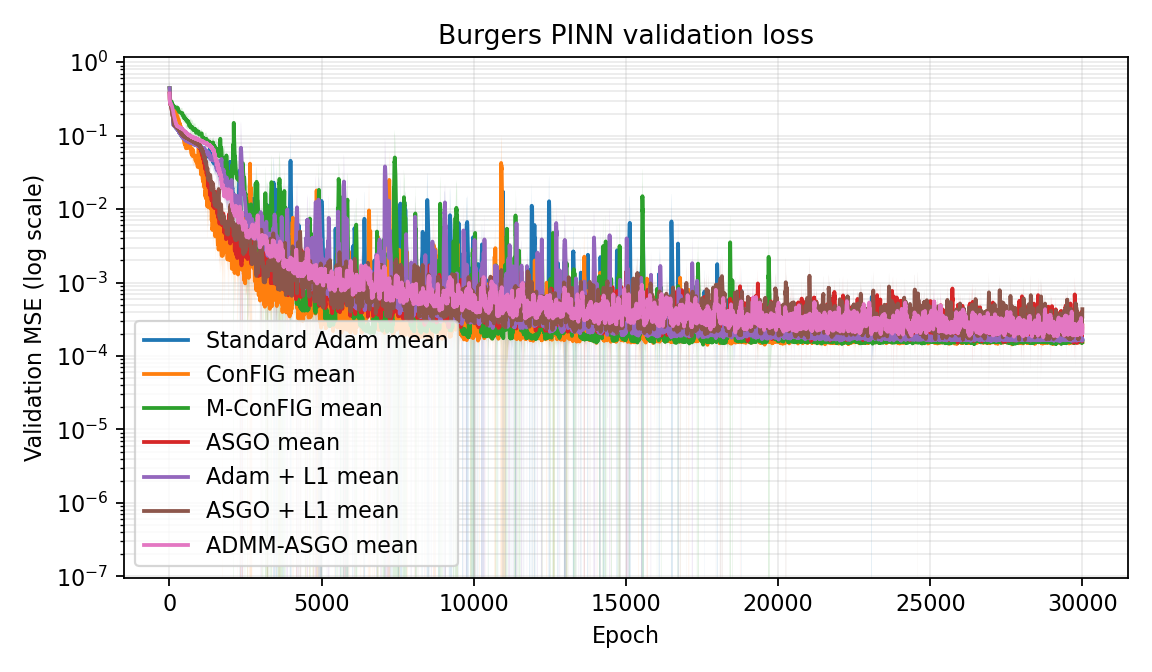
\includegraphics[width=0.92\textwidth,height=0.58\textheight,keepaspectratio]{../../report_assets/Experiment2_ADMM_ASGO/burgers_validation_loss.png}
\caption{Burgers validation loss}
\end{figure}


精度-稀疏度图如下。只有 ADMM-ASGO 产生明显稀疏率，其余方法严格零权重比例均为 0。

\begin{figure}[H]
\centering
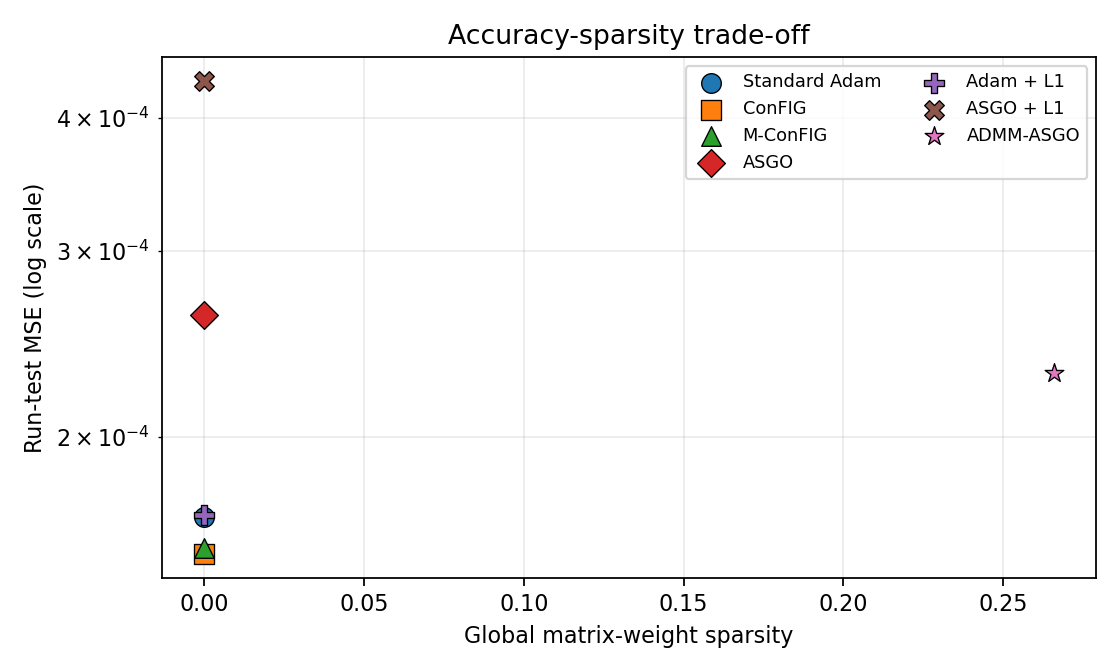
\includegraphics[width=0.92\textwidth,height=0.58\textheight,keepaspectratio]{../../report_assets/Experiment2_ADMM_ASGO/burgers_accuracy_sparsity.png}
\caption{Accuracy-sparsity trade-off}
\end{figure}


全局稀疏率图如下。

\begin{figure}[H]
\centering
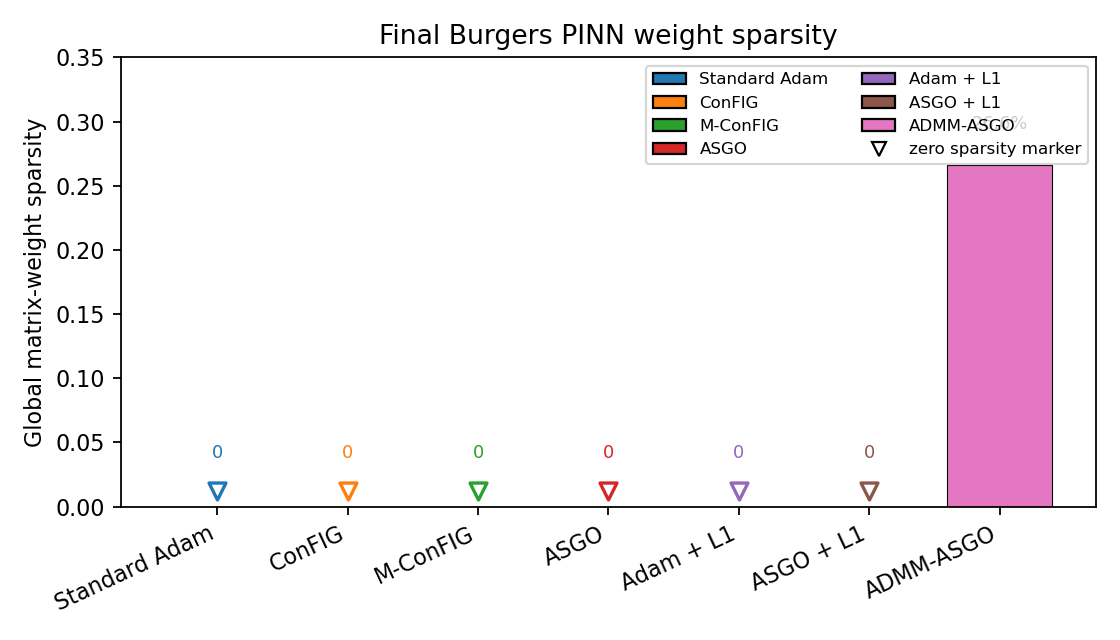
\includegraphics[width=0.92\textwidth,height=0.58\textheight,keepaspectratio]{../../report_assets/Experiment2_ADMM_ASGO/burgers_weight_sparsity.png}
\caption{Global sparsity}
\end{figure}


逐层稀疏率图如下。

\begin{figure}[H]
\centering
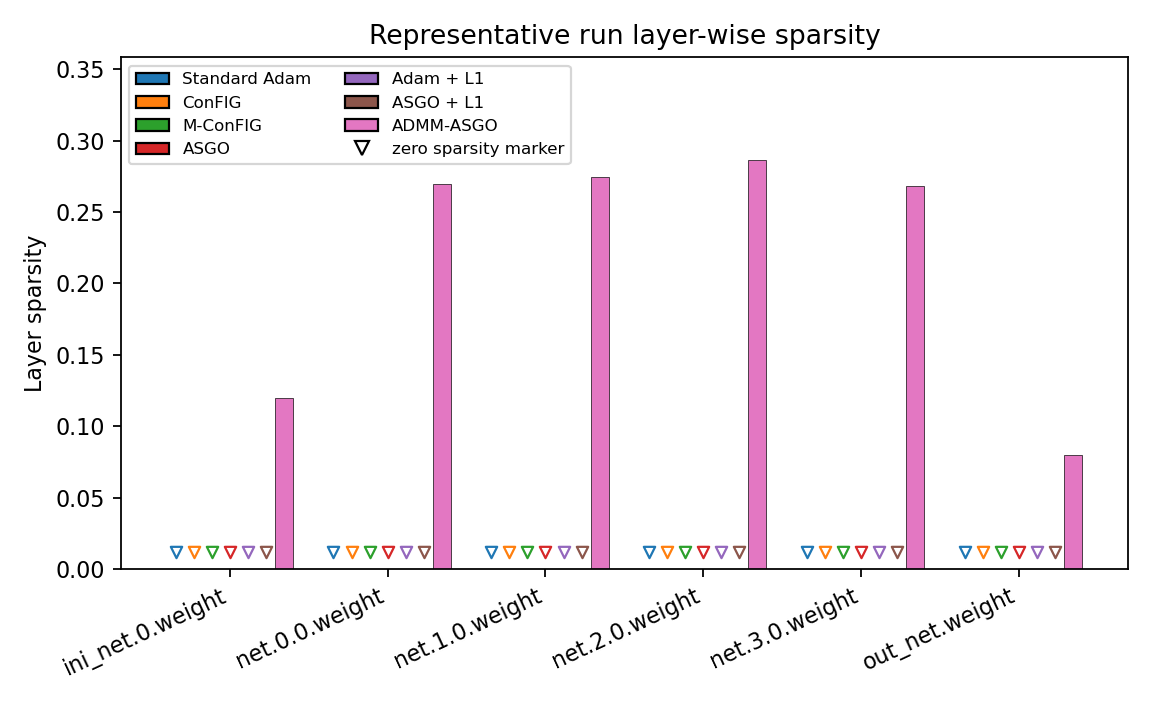
\includegraphics[width=0.92\textwidth,height=0.58\textheight,keepaspectratio]{../../report_assets/Experiment2_ADMM_ASGO/burgers_layer_sparsity.png}
\caption{Layer sparsity}
\end{figure}


Burgers 预测和误差热力图如下。

\begin{figure}[H]
\centering
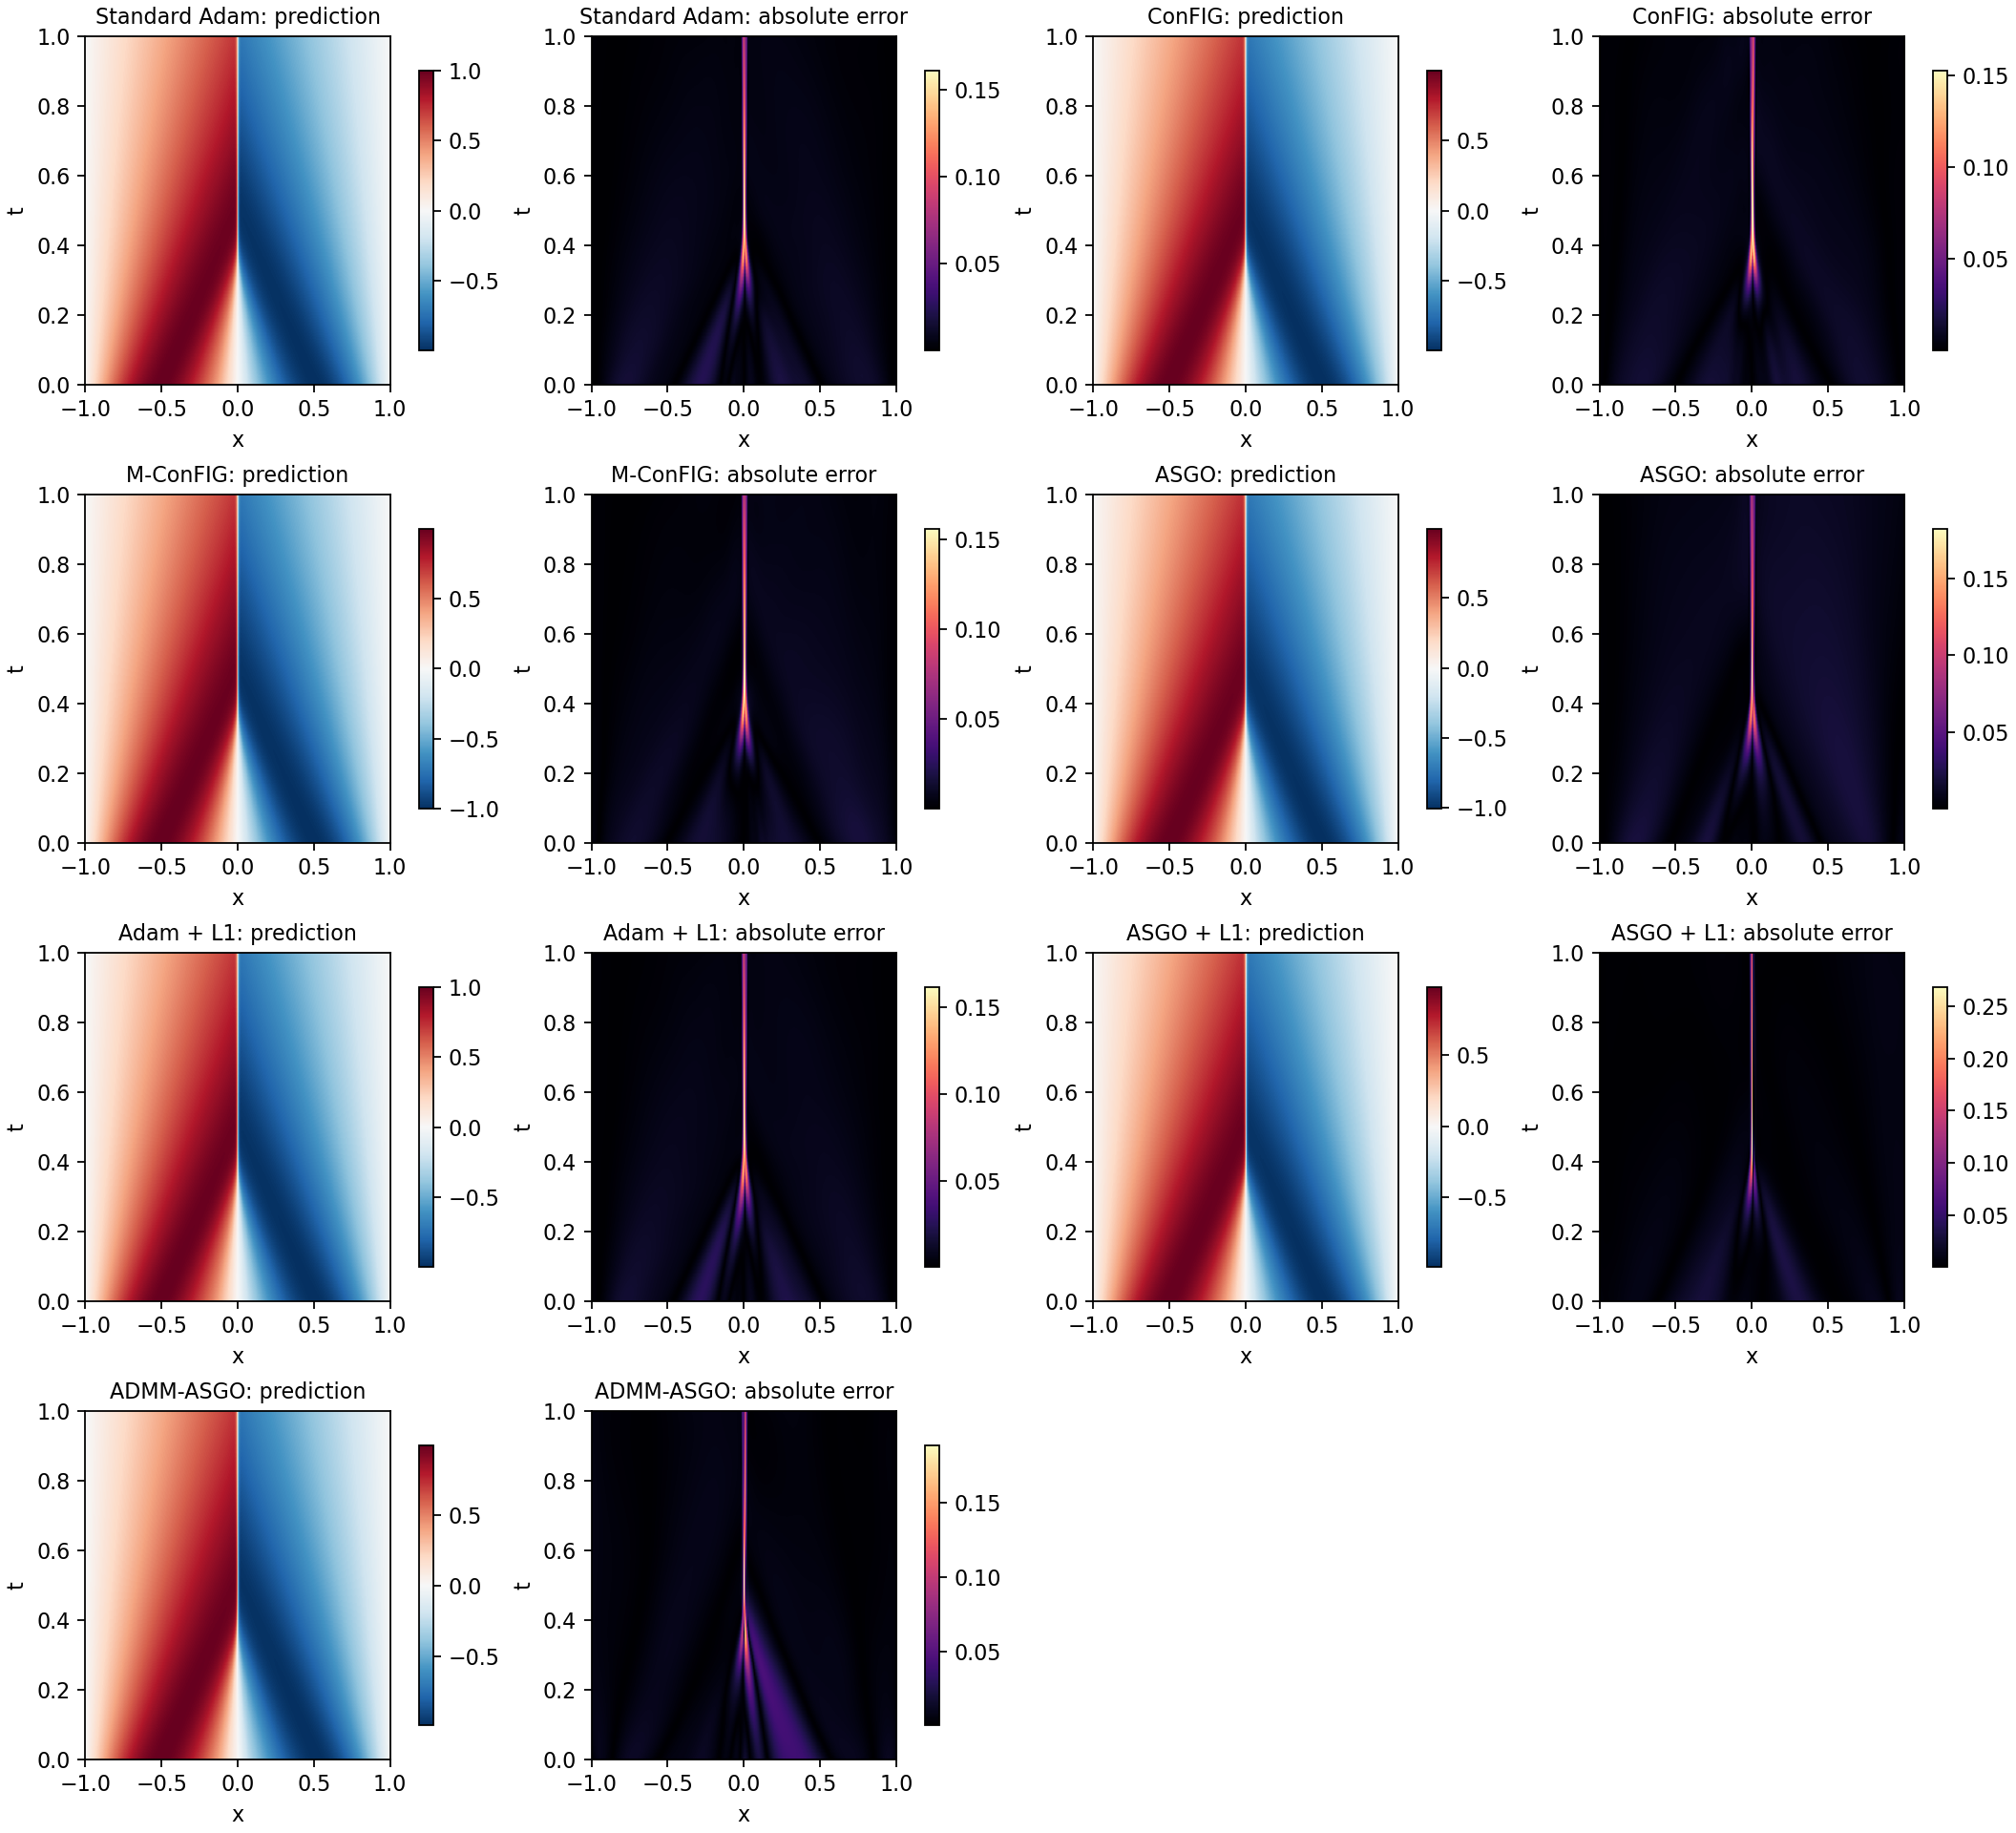
\includegraphics[width=0.92\textwidth,height=0.58\textheight,keepaspectratio]{../../report_assets/Experiment2_ADMM_ASGO/burgers_predictions_errors.png}
\caption{Predictions and errors}
\end{figure}


参考解热力图如下。

\begin{figure}[H]
\centering
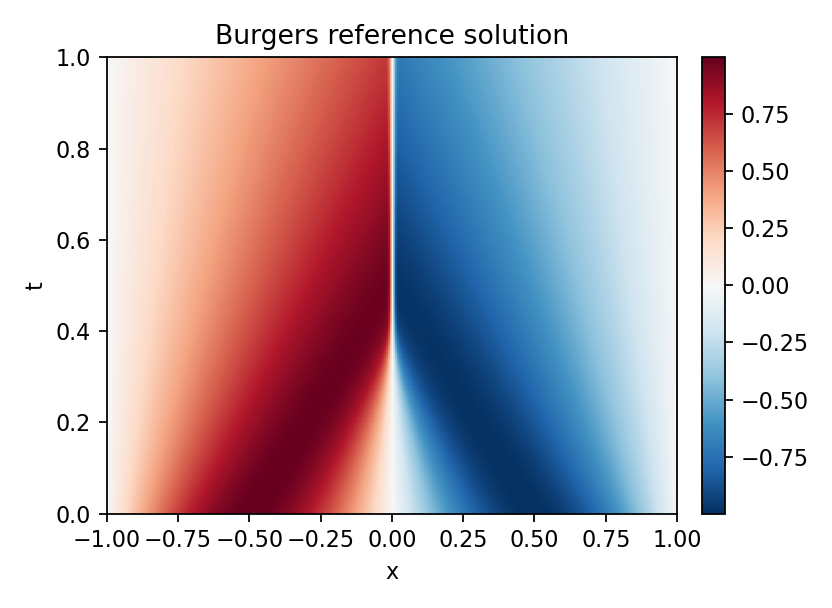
\includegraphics[width=0.92\textwidth,height=0.58\textheight,keepaspectratio]{../../report_assets/Experiment2_ADMM_ASGO/burgers_reference_solution.png}
\caption{Reference solution}
\end{figure}


\section{结果分析与理解}

\subsection{普通 L1 正则为什么没有产生严格零权重}

Adam + L1 的 run-test MSE 为 $1.6884\times 10^{-4}$，与 Standard Adam 的 $1.6799\times 10^{-4}$ 非常接近，但稀疏率仍为 0。ASGO + L1 的稀疏率同样为 0。这说明在本实验的有限训练步中，直接把 L1 范数加到损失函数中，确实能给权重一个向 0 收缩的梯度，但不会自动执行“截断到 0”的操作。

从优化角度看，L1 正则的近端算子是软阈值，而普通梯度法并没有显式调用这个近端步骤。因此参数可能变小，却很难精确等于 0。这个结果正好说明 ADMM 变量分裂的必要性：如果实验目标是得到严格稀疏网络，而不仅是小权重网络，那么需要近端步骤或显式剪枝机制。

\subsection{ADMM-ASGO 验证了严格稀疏化想法}

ADMM-ASGO 得到 26.58\% 的矩阵权重稀疏率，非零矩阵权重约为 7452 个。这是本实验最重要的现象：在不改变 PINN 数据和网络结构的情况下，只通过 ADMM 的 $z$ 子问题软阈值步骤，就能得到严格零权重。

逐层结果表明，中间隐藏层承担了主要压缩量。输入层只有 12.00\% 稀疏率，输出层只有 8.00\% 稀疏率，而四个隐藏层均在 26.80\% 到 28.68\% 之间。这种分布是合理的：输入输出层维度较小，直接决定坐标到解值的映射；隐藏层矩阵更大，存在更多冗余自由度，因此更适合被稀疏化。

\subsection{稀疏化带来的精度折中}

ADMM-ASGO 的 run-test MSE 为 $2.3000\times 10^{-4}$，高于 Standard Adam 的 $1.6799\times 10^{-4}$、ConFIG 的 $1.5516\times 10^{-4}$ 和 M-ConFIG 的 $1.5714\times 10^{-4}$。这说明稀疏约束确实会给 PINN 拟合带来压力，尤其是 Burgers 方程存在较明显的非线性和局部变化，过度压缩权重可能削弱网络表达能力。

但是 ADMM-ASGO 的误差仍与其他方法处在同一数量级，没有发生发散或物理解完全失效。这支持一个更谨慎也更真实的结论：ADMM-ASGO 在本实验中不是“更准”的方法，而是“用可接受的精度损失换取严格稀疏性”的方法。它验证了稀疏化与物理残差拟合之间存在可调折中。

\subsection{ASGO 在本任务中的表现}

ASGO 的 best validation MSE 为 $1.2288\times 10^{-4}$，是所有方法中最低的 best validation MSE，但 final validation MSE 和 run-test MSE 为 $2.6053\times 10^{-4}$。这说明 ASGO 在训练过程中曾找到很好的参数区域，但后期稳定性不如 ConFIG/M-ConFIG。ASGO + L1 的 best validation MSE 也较好，但 final MSE 波动更大。

这提示在 PINN 任务中，结构化优化器的收益可能与学习率、预条件强度、训练后期调度和正则项强度密切相关。本实验为了控制变量，没有对 ASGO 做大规模超参数搜索。因此报告中的 ASGO 结果主要用于证明它能被接入 ADMM 子问题，而不是证明其在 Burgers PINN 上已经达到最优调参状态。

\subsection{ADMM residual 的含义}

ADMM-ASGO 的 primal residual 为 $2.9150\times 10^{-2}$，dual residual 为 $2.5794\times 10^{-4}$。primal residual 衡量 $\theta$ 与 $z$ 的一致性，dual residual 衡量 $z$ 变量相邻迭代的变化。dual residual 较小说明稀疏变量后期变化稳定；primal residual 不为 0 则说明在非凸 PINN 和单步 inexact ADMM 设置下，$\theta$ 子问题没有被精确求解，一致性约束并未完全收敛。

这与本文方法设计一致：我们使用的是面向神经网络训练的非精确随机 ADMM，而不是每轮精确求解凸子问题的经典 ADMM。对本实验而言，更重要的是训练过程稳定、最终保存模型稀疏、误差可接受。

\section{创新点与局限性}

本实验的改进点可以概括为三点：

\begin{enumerate}
\item 将 ASGO 的结构化矩阵优化嵌入 ADMM 的 $\theta$ 子问题；
\item 用 ADMM 软阈值步骤显式产生严格零权重，而不是只依赖普通 L1 梯度惩罚；
\item 在 Burgers PINN 中同时报告精度、速度、全局稀疏率、逐层稀疏率和 ADMM residual，使“精度-稀疏度折中”可以被直接观察。
\end{enumerate}

实验的局限性也很明确：

\begin{enumerate}
\item 只在 Burgers 1D PINN 上验证，没有扩展到更多 PDE；
\item $\lambda$ 和 $\rho$ 只使用一组主实验参数，没有完整画出 Pareto 曲线；
\item ASGO 在本任务中没有做充分调参，后期误差波动较大；
\item ADMM-ASGO 当前只稀疏化 \texttt{Linear.weight}，没有研究 bias、卷积层或更复杂结构。
\end{enumerate}

这些局限不影响本实验的主要结论，因为本文目标不是刷最高精度，而是验证 ADMM 处理非光滑 L1 项、ASGO 处理光滑矩阵权重子问题这一组合思路。

\section{结论}

本实验完成了从理论推导、代码实现到正式多随机种子验证的完整流程。理论上，报告推导了三个 L1 正则/约束问题的 ADMM 公式，说明 ADMM 如何把光滑目标与非光滑 L1 项分开处理。实现上，实验在 Burgers PINN 中新增 ASGO 适配层、普通 L1 基线和 ADMM-ASGO 稀疏训练器。实验上，30000 epoch、3 个随机种子的结果表明：

\begin{enumerate}
\item Standard Adam、ConFIG、M-ConFIG、ASGO、Adam + L1、ASGO + L1 均没有产生严格零矩阵权重；
\item ADMM-ASGO 得到 26.58\% 的严格矩阵权重稀疏率；
\item ADMM-ASGO 的 run-test MSE 为 $2.3000\times 10^{-4}$，虽高于最强精度基线，但仍处于同一数量级；
\item 普通 L1 正则不能替代 ADMM 软阈值步骤，后者才是严格稀疏性的直接来源。
\end{enumerate}

因此，本实验验证了预设想法：将 ASGO 的结构化梯度优化能力嵌入 ADMM 的光滑子问题，并用软阈值显式处理 L1 非光滑正则，可以在 PINN 中得到可复现的严格稀疏模型。最终结论应理解为“ADMM-ASGO 提供了一种可解释的稀疏化训练机制”，而不是“ADMM-ASGO 在精度上超过所有优化器”。

后续工作可以继续对 $\lambda$ 与 $\rho$ 做系统消融，研究稀疏率和 MSE 的 Pareto 前沿；也可以把 ADMM 稀疏化与 ConFIG/M-ConFIG 的梯度冲突处理结合，进一步同时优化物理约束拟合和模型压缩。

\newpage
\section{附录：关键算法代码}

本附录只列出实验二讲解中最关键的实现片段。完整实现分布在稀疏训练器、实验运行脚本和结果分析脚本中；附录保留的是讲解 ADMM-ASGO 方法时最需要展示的代码。这些片段对应报告正文中的三个核心问题：如何产生严格零权重，如何把 ASGO 只作用在矩阵权重上，以及 ADMM 的 $\theta/z/u$ 三步如何在训练循环中实现。

\subsection{A.1 软阈值算子与稀疏参数选择}

\texttt{soft\_threshold} 是 L1 近端步骤的核心。若某个元素的绝对值不超过阈值，它会被直接置为 0；因此 ADMM-ASGO 的严格稀疏性来自这里，而不是来自普通梯度下降。

\begin{lstlisting}
def soft_threshold(values: torch.Tensor, threshold: float) -> torch.Tensor:
    """Elementwise proximal operator for threshold * ||x||_1."""
    return torch.sign(values) * torch.clamp(torch.abs(values) - threshold, min=0.0)


def sparse_named_parameters(network: torch.nn.Module) -> list[tuple[str, torch.nn.Parameter]]:
    """Only matrix weights are managed by L1/ADMM sparsity."""
    return [
        (name, param)
        for name, param in network.named_parameters()
        if param.requires_grad and param.ndim >= 2
    ]


def l1_penalty(network: torch.nn.Module) -> torch.Tensor:
    params = sparse_named_parameters(network)
    if not params:
        return torch.zeros((), device=next(network.parameters()).device)
    return torch.stack([param.abs().sum() for _name, param in params]).sum()
\end{lstlisting}

\subsection{A.2 ASGO 与 Adam 的混合优化器}

ASGO 适合二维矩阵权重，bias 和一维参数不适合做矩阵预条件。因此实验中对 \texttt{Linear.weight} 使用 ASGO，对 bias 使用 Adam。这一设计对应正文中的“ASGO 求解 ADMM 的光滑 $\theta$ 子问题”。

\begin{lstlisting}
class HybridOptimizer:
    """Wrap ASGO for matrix weights and Adam for bias/1-D parameters."""

    def __init__(self, optimizers: list[torch.optim.Optimizer]) -> None:
        self.optimizers = optimizers
        self.param_groups = []
        for optimizer in optimizers:
            self.param_groups.extend(optimizer.param_groups)

    def zero_grad(self) -> None:
        for optimizer in self.optimizers:
            optimizer.zero_grad()

    def step(self) -> None:
        for optimizer in self.optimizers:
            optimizer.step()


class ASGOTrainerBasis(StandardTrainerBasis):
    def get_optimizer(self, network):
        matrix_params = [param for _name, param in sparse_named_parameters(network)]
        adam_params = [
            param for _name, param in network.named_parameters()
            if param.requires_grad and param.ndim < 2
        ]
        optimizers = []
        if matrix_params:
            optimizers.append(LocalASGO(matrix_params, learning_rate=self.configs.lr))
        if adam_params:
            optimizers.append(torch.optim.Adam(adam_params, lr=self.configs.lr))
        return HybridOptimizer(optimizers)
\end{lstlisting}

\subsection{A.3 ADMM-ASGO 训练器核心循环}

下面代码对应 ADMM 的三步。\texttt{train\_step} 在原 PINN loss 上加入 $\theta$ 子问题的二次惩罚项；\texttt{event\_after\_training\_iteration} 执行软阈值 $z$ 更新和对偶变量 $u$ 更新；训练结束时把稀疏副本 \texttt{z} 写回网络权重，使保存的模型本身就是稀疏模型。

\begin{lstlisting}
class ADMMASGOTrainerBasis(ASGOTrainerBasis):
    def event_before_training(self, network):
        super().event_before_training(network)
        self._admm_params = sparse_named_parameters(network)
        self._admm_z = {name: param.detach().clone() for name, param in self._admm_params}
        self._admm_u = {name: torch.zeros_like(param) for name, param in self._admm_params}

    def train_step(self, network, batched_data, idx_batch, num_batches, idx_epoch, num_epoch):
        total_loss = super().train_step(network, batched_data, idx_batch, num_batches, idx_epoch, num_epoch)
        penalty_terms = []
        for name, param in self._admm_params:
            z = self._admm_z[name].to(device=param.device, dtype=param.dtype)
            u = self._admm_u[name].to(device=param.device, dtype=param.dtype)
            penalty_terms.append(torch.sum((param - z + u) ** 2))
        admm_penalty = 0.5 * self.configs.admm_rho * torch.stack(penalty_terms).sum()
        return total_loss + admm_penalty

    @torch.no_grad()
    def event_after_training_iteration(self, network, idx_epoch, idx_batch):
        threshold = self.configs.admm_lambda / self.configs.admm_rho
        primal, dual = [], []
        for name, param in self._admm_params:
            z_prev = self._admm_z[name].to(device=param.device, dtype=param.dtype)
            u_prev = self._admm_u[name].to(device=param.device, dtype=param.dtype)

            z_next = soft_threshold(param + u_prev, threshold)
            u_next = u_prev + param - z_next

            primal.append(torch.sum((param - z_next) ** 2))
            dual.append(torch.sum((self.configs.admm_rho * (z_next - z_prev)) ** 2))
            self._admm_z[name] = z_next.detach().clone()
            self._admm_u[name] = u_next.detach().clone()

        self._last_admm_primal_residual = float(torch.sqrt(torch.stack(primal).sum()).cpu())
        self._last_admm_dual_residual = float(torch.sqrt(torch.stack(dual).sum()).cpu())

    @torch.no_grad()
    def event_after_training(self, network):
        for name, param in self._admm_params:
            param.copy_(self._admm_z[name].to(device=param.device, dtype=param.dtype))
\end{lstlisting}

\newpage
\section{参考文献}

[1] Pablo Villalobos, Jaime Sevilla, Lennart Heim, Tamay Besiroglu, Marius Hobbhahn, Anson Ho. Will we run out of data? Limits of LLM scaling based on human-generated data. arXiv:2211.04325, 2022. \url{https://arxiv.org/abs/2211.04325}

[2] Kang An, Yuxing Liu, Rui Pan, Yi Ren, Shiqian Ma, Donald Goldfarb, Tong Zhang. ASGO: Adaptive Structured Gradient Optimization. NeurIPS 2025. \url{https://openreview.net/forum?id=fru52tkjHf}

[3] Shenglong Zhou, Ouya Wang, Ziyan Luo, Yongxu Zhu, Geoffrey Ye Li. Preconditioned inexact stochastic ADMM for deep models. Nature Machine Intelligence, 8:234-245, 2026. \url{https://www.nature.com/articles/s42256-026-01182-3}

[4] Maziar Raissi, Paris Perdikaris, George Em Karniadakis. Physics-informed neural networks: A deep learning framework for solving forward and inverse problems involving nonlinear partial differential equations. Journal of Computational Physics, 2019.

[5] Tianhe Yu, Saurabh Kumar, Abhishek Gupta, Sergey Levine, Karol Hausman, Chelsea Finn. Gradient Surgery for Multi-Task Learning. NeurIPS 2020.

\end{document}
